\chapter{Results}\label{chapter:Results}

In this chapter, we summarize our results comparing different DDPG algorithms specified before in Chapters \ref{chapter:DDPGFuncs} , \ref{chapter:ShockBuffer}, and \ref{chapter:Estimates}.

We first provide an overall view of the results across all the configurations we have tested. We then drill down to the performance of the algorithm under different market conditions. Some of the metrics we tested in this case are
\begin{itemize}
    \item Utility functions of wealth for the investor.
    \item Mean return ($\mu$) and volatility ($\sigma$) of the risky asset.
    \item Risk aversion factor $b$ of the investor in the case of power utility.
    \item Number of time steps (time discretization) in an episode
\end{itemize}

We proceed then to do a hyper parameter search on the tunable parameters in the different algorithms and then make inferences on the optimal hyper parameter configuration to improve our performance. Some of the hyper parameters we considered are
\begin{itemize}
\item $\tau$ -  target learning rate 
\item Noise scale to the exploration part in DDPG.
\item Number of episodes
\item Batch size
\item Number of grid points on DDPG Estimate 
\item Batch size $|B_p|=m$, for the log  returns in DDPG Shock Buffer 
\end{itemize}

We found out that in particular, Shock Buffer (Chapter \ref{chapter:ShockBuffer}) and Estimates (Chapter \ref{chapter:Estimates}) were robust and as we increased the number of sampled log returns of the shock $m$ and the number of partitions (also $m$) respectively, the accuracy also significantly increased. We repeated the experiments by increasing the number of time steps and across different model parameters for the robust version and found out that the results were stable.


\section{Performance Analysis}

We define four benchmarks  to summarize the performance analysis of our experiments. 
\begin{itemize}
    \item \textbf{Accuracy} as defined by the following equations
    \begin{equation}
        Error_{actual} = \frac{|\pi^* - a^{\phi}|}{\pi^*}
    \end{equation}
    \begin{equation}\label{equation:error}
            Error_{Normalized} = 
        \begin{cases}
          Error_{actual} \quad  Error_{actual} \leq 1 \\
          1 \quad otherwise
        \end{cases}
    \end{equation}
    \begin{equation}
        Accuracy = 1 - Error_{Normalized}.
    \end{equation}
    \item \textbf{Signed Loss} as defined by
    \begin{equation}
        Signed Loss = \pi^* - a^\phi.
    \end{equation}
    \item \textbf{Absolute Loss} as defined by
         \begin{equation}
        Absolute Loss = |\pi^* - a^\phi|.
    \end{equation}
    \item \textbf{Variance} as defined by
             \begin{equation}
                Variance = \frac{1}{100}\big {\Sigma_{i=0}^{99}} \left(a^{\phi^{(n-i)}}-\frac{1}{100}\Sigma_{j=0}^{99}a^{\phi^{(n-j)}}\right)^2,
    \end{equation}
    where $n$ is the last recent update to the algorithm
    
\end{itemize}

Going forward in this chapter, we refer to DDPG Functions, DDPG Shock Buffer and DDPG Estimates as DDPG, Shock Buffer and Estimates, respectively.
\pagebreak
\subsection{Accuracy and Losses - Overview}
We conducted a variety of experiments, with different time steps and environment parameters. The different configuration of these parameters are shown in Table \ref{table:config_overall}. In the table, Grid Points is only applicable to DDPG Estimate,  and Shock Buffer Size is only applicable to DDPG Shock  Buffer. 

\begin{table}[]
\caption{Overview configuration} \label{table:config_overall}
\begin{tabular}{||p{3cm}|p{2cm}||p{2cm}|p{2cm}||p{2cm}|p{2cm}||}
\hline
\textbf{Environment Parameter} & \textbf{Sampled values} &\textbf{DDPG}\linebreak \textbf{Parameter}& \textbf{Values} & \textbf{DDPG}\linebreak \textbf{Parameter} & \textbf{Values}\\
\hline

$\mu \in [0,1]$          & [0.07,0.955] & Version & DDPG, Shock Buffer, Estimates & Batch Size          & 1024 \\
\hline
$\sigma \in [0,1]$       & [0.1,1.4] & Grid Points &[8,1024]& Batch Size Growth & None and Linear \\
\hline
\Delta t          & [0.01,0.2] & Shock Buffer Size & [8,1024] & &\\
\hline
$v_0 \in (0,1]$        & [0.1,0.9] & Noise \linebreak  Decay       & Linear and None & & \\
\hline
Utility     & power and log & Noise \linebreak  Scale       & [0.1,5] &&  \\
\hline
$b \in [-10,1) \backslash \{0\}$ & [-9.0,0.95]  & $\tau$& $5.10^{-4}$ && \\
\hline
            T&1  &$\tau$ decay         & Linear and None && \\
\hline
            $r_c$&0  & Buffer Length     & [$10^{4}$, $10^{5}$] && \\
\hline
\end{tabular}
\end{table}



    \begin{figure}[!tbp]
  \subfloat[Box plot comparison ][Box plot comparison for all DDPG algorithms - Accuracy]{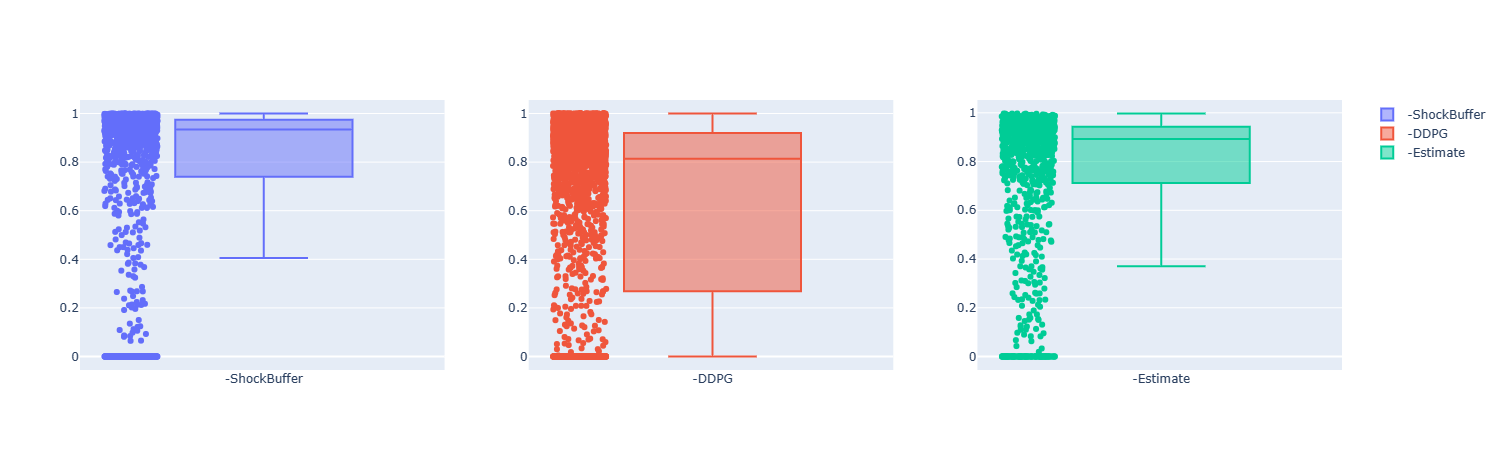
\includegraphics[width=1\textwidth,height=0.22\textheight]{figures/Results/BoxPlot_All.png}}
  \vfill
  \subfloat[Table Analysis][Tabular description of algorithms (accuracy)]{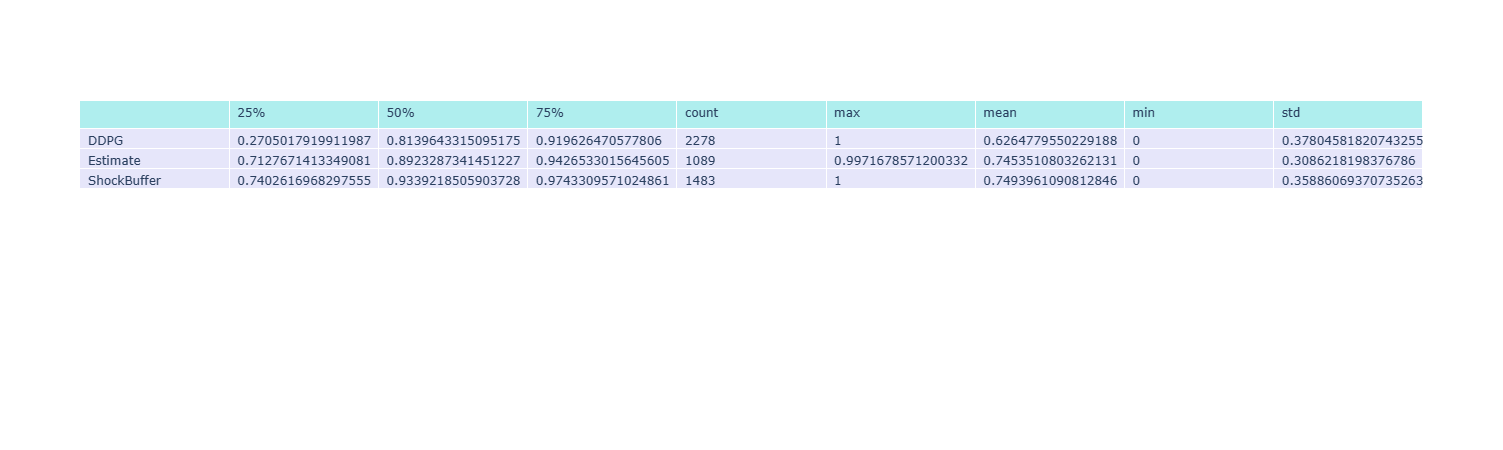
\includegraphics[width=1\textwidth,height=0.22\textheight]{figures/Results/df_BP_all.png}}
  \vfill
    \subfloat[Box plot comparison ][Box plot comparison for all DDPG algorithms - signed loss ]{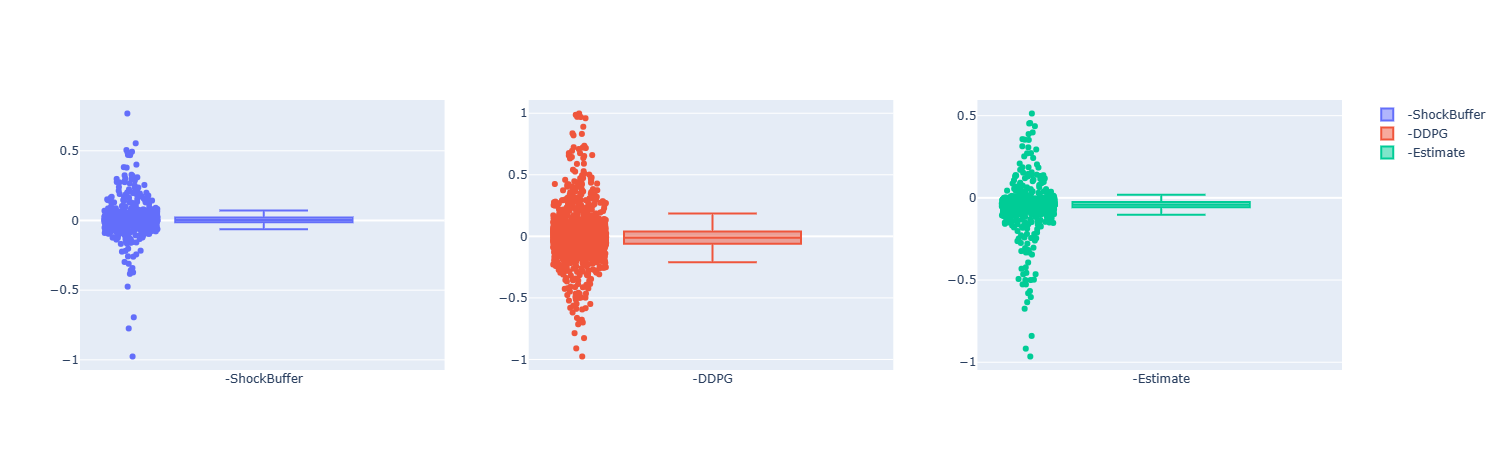
\includegraphics[width=1\textwidth,height=0.22\textheight]{figures/Results/BoxPlot_SL_All.png}}
  \vfill
  \subfloat[Table Analysis][Tabular description of algorithms (signed loss)]{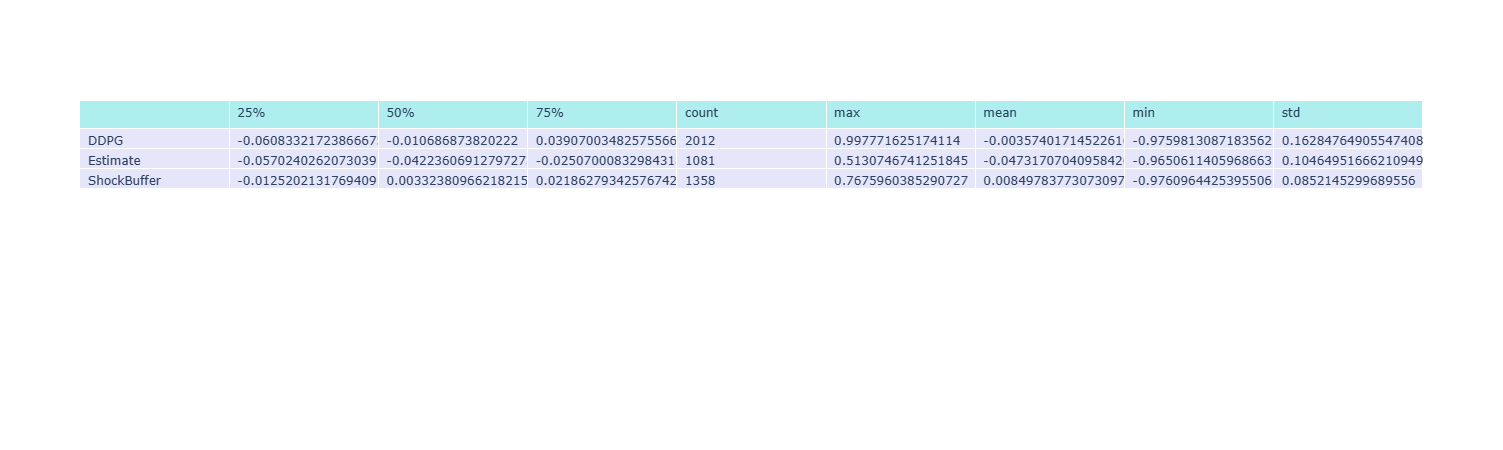
\includegraphics[width=1\textwidth,height=0.2\textheight]{figures/Results/df_BP_SL_all.png}}
  
  \caption{ Performance analysis}
  \label{fig:results:performance_analysis_all}
\end{figure}

In Figure \ref{fig:results:performance_analysis_all}, we filtered experiments, with accuracy at least greater than 0\% and removed the simulations where gradients exploded. The number of experiments were different in different versions for many reasons. Some experiments (noise scale analysis) were only conducted in 1 version of the solution (DDPG, Shock Buffer or Estimates). We started off with DDPG, and developed the other versions later so we had more experiments on DDPG compared to the rest.

From Figure \ref{fig:results:AbsAExAnalysis}, it appears that Shock Buffer and Estimates performed (in terms of accuracy) much better compared to DDPG.    All quantiles as well as the mean accuracy are higher.

Comparing Shock Buffer and Estimates, we see that Shock Buffer generally performs better. The standard deviation of accuracy for Shock Buffer is however higher compared to Estimates. In our experiments we noted that Shock Buffer simulations were quite "noisy" in convergence compared to Estimates. The sample variance in the optimal action in the experiments we conducted were lower for Estimates (2.8e-7) compared to Shock buffer (7.8e-6) at the 50th percentile.

Looking at the box plot of the signed loss in Figure \ref{fig:results:performance_analysis_all}, we see an interesting pattern for Estimates. The loss is mostly negative. which means the calculated optimal action value is lower than the optimal value. Here it seems like Estimates yields biased values for $a^*$ compared to the other versions which have a median signed loss of approximately 0.

Further, we plotted the mean absolute loss across bins of the expected optimal action constrained between 0 and 1 in Figure \ref{fig:results:AbsAExAnalysis}. 
\begin{figure}[htpb]
  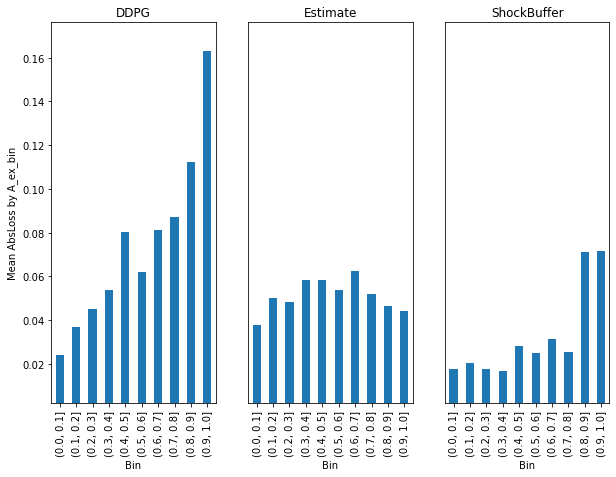
\includegraphics[width=1\textwidth,height=6cm]{figures/Results/AbsLossA_ex.png}
  \caption[Absolute loss analysis]{Absolute loss analysis} \label{fig:results:AbsAExAnalysis}
\end{figure}

In DDPG and Shock Buffer we see that as the true value of the optimal action, $a^*$  increases,  the absolute losses are much higher compared to the other intervals. However for Estimates, the absolute losses seem to be more robust in the interval [0,1].
\pagebreak

\section{Environment search}

Next we also tried to do an environment search across different model parameters and across different utility functions. The procedure for selecting the parameters is listed in Algorithm \ref{algo:EnvSearch}
\begin{algorithm}
\caption{Generate environment parameters procedure} \label{algo:EnvSearch}
\begin{algorithmic}[1]
\Require
\Statex N \Comment{Number of observations}
\Statex
\State $i \gets 0$

\While {$i<N$}
    \State $\mu \gets UniformDistribution(0,1)$
    \State $\sigma \gets UniformDistribution(0,1)$
    \State $b \gets UniformDistribution(-10,1)$
    \State  $a^*_{log} \gets \mu/\sigma^2$
    \State $a^*_{pow} \gets \mu/((1-b)\sigma^2)$
    \If {$a^*_{log} < 1$ and $a^*_{pow} < 1$}
        \State Add environment parameters \{$\mu,\sigma,b$\}
        \State $i \gets i+1$
    \EndIf
\EndWhile
\end{algorithmic}
\end{algorithm}

We sampled uniform random variables in the range [0,1] for $\mu$ and $\sigma$. For b we used a uniform distribution in the range [-10,1]. We also made sure that, expected optimal action, $a^*$ was within the range [0,1]  

The configuration for these experiments are shown in Table \ref{table:config_env}

\begin{table}[]
\caption{Configuration - Environment Analysis} \label{table:config_env}
\begin{tabular}{||p{3cm}|p{2cm}||p{2cm}|p{2cm}||p{2cm}|p{2cm}||}
\hline
\textbf{Environment Parameter} & \textbf{Sampled values} &\textbf{DDPG}\linebreak \textbf{Parameter}& \textbf{Values} &\textbf{DDPG}\linebreak \textbf{Parameter} & \textbf{Values}\\
\hline

$\mu \in [0,1]$           & \textbf{[0.07,0.955]} & Version & DDPG, Shock Buffer, Estimates & Batch Size          & 1024 \\
\hline
$\sigma\in [0,1]$        & \textbf{[0.1,1.0]} & Grid Points &20 (Estimate)& Batch Size Growth & None \\
\hline
\Delta t          & 0.2 & Shock Buffer Size & 8 (Shock Buffer)& &\\
\hline
$v_0$        & 1 & Noise \linebreak  Decay       & Linear & & \\
\hline
Utility     & power and log & Noise \linebreak  Scale       & 1 &&  \\
\hline
$b \in [-10,1) \backslash \{0\}$ & [-9,0.95]  & $\tau$& $5.10^{-4}$ && \\
\hline
            T&1  &$\tau$ decay         & Linear && \\
\hline
            $r_c$&0  & Buffer Length     & $10^{4}$ && \\
\hline
\end{tabular}
\end{table}


The results are shown in Figures \ref{fig:results:AHMPU}, \ref{fig:results:AHMLU} and \ref{fig:results:AHMA}. The lower triangle in these plots is empty because of the way the parameters were chosen with the constraint on optimal action values, $a^*$ being in [0,1].

\begin{figure}[htpb]
  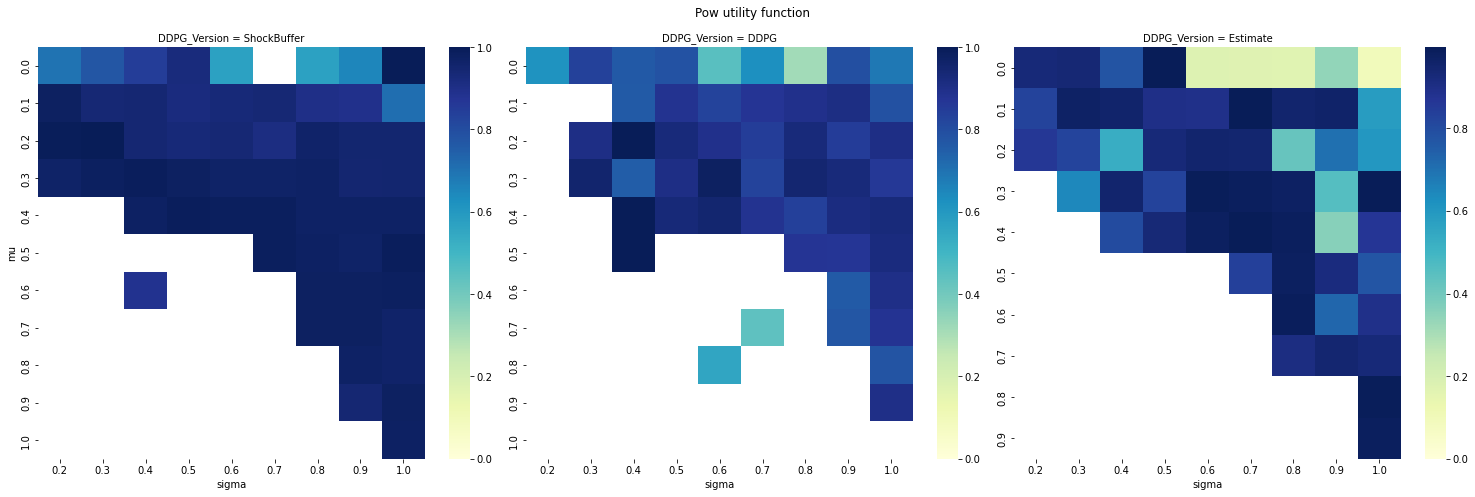
\includegraphics[width=1\textwidth,height=6cm]{figures/Results/Heatmap1.png}
  \caption[Accuracy heat map - Power utility]{Accuracy heat map - Power utility} \label{fig:results:AHMPU}
\end{figure}
\begin{figure}[htpb]
    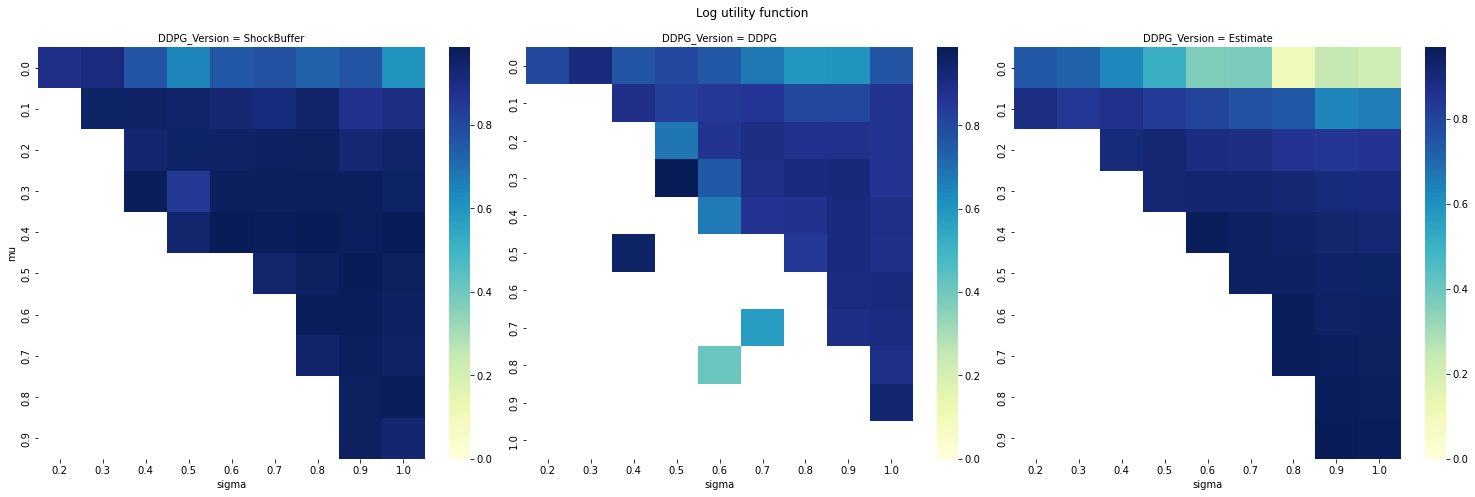
\includegraphics[width=1\textwidth,height=6cm]{figures/Results/Heatmaplog.png}
  \caption[Accuracy heat map - Log]{Accuracy heat map - Log utility} \label{fig:results:AHMLU}
\end{figure}
\begin{figure}[htpb]
    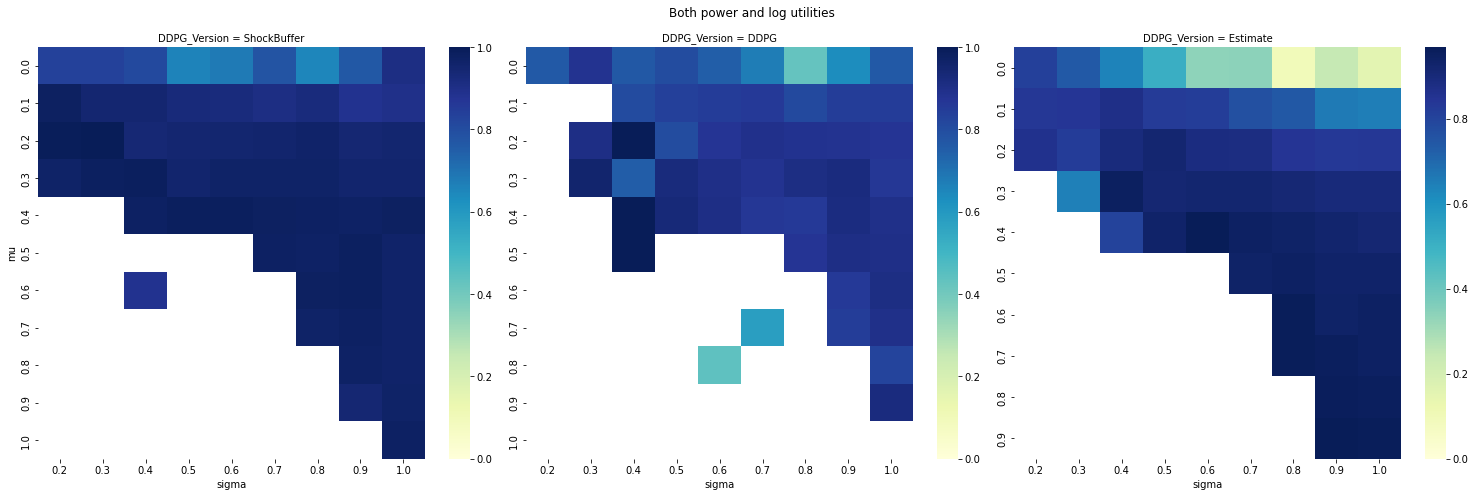
\includegraphics[width=1\textwidth,height=6cm]{figures/Results/heatmap_both.png}
  \caption[Accuracy heat map - All]{Accuracy heat map for both utility functions} \label{fig:results:AHMA}
\end{figure}

We see that Shock Buffer and Estimates have better accuracy in most of the regions in the heatmap. We also observe that there are no particular regions in the grid, where the accuracy is markedly different (for any of the algorithms). We do note that when $\mu$ is small, the accuracy is lower. However, the expected optimal action for both utility functions are directly proportional to $\mu$. Hence, when the optimal action value is also very small, the accuracy may be significantly impacted even for minor perturbations from the theoretical values.

\pagebreak

\subsection{Risk Aversion analysis for Power Utility}
We also analyzed with a number of values for $b$, the risk aversion factor for the power utility function.  We expect that as b approaches 1, the absolute losses should increase as the true optimal allocation $\pi^*$ also increases. 

The configuration for these experiments are shown in Table \ref{table:config_b}  and the results are shown in Figure \ref{fig:results:bA}.

\begin{table}[]
\caption{Configuration - Environment Analysis - Risk aversion} \label{table:config_b}
\begin{tabular}{||p{3cm}|p{2cm}||p{2cm}|p{2cm}||p{2cm}|p{2cm}||}
\hline
\textbf{Environment Parameter} & \textbf{Sampled values} &\textbf{DDPG}\linebreak \textbf{Parameter}& \textbf{Values} &\textbf{DDPG}\linebreak \textbf{Parameter} & \textbf{Values}\\
\hline

$\mu \in [0,1]$          & [0.07,0.955] & Version & DDPG, Shock Buffer, Estimates & Batch Size          & 1024 \\
\hline
$\sigma \in [0,1]$       & [0.1,1.0] & Grid Points &20 (Estimate)& Batch Size Growth & None \\
\hline
\Delta t          & 0.2 & Shock Buffer Size & 8 (Shock Buffer)& &\\
\hline
$v_0$        & 1 & Noise \linebreak  Decay       & Linear & & \\
\hline
Utility     & power  & Noise \linebreak  Scale       & 1 &&  \\
\hline
$\mathbf{b \in [-10,1) \backslash \{0\}}$           & \textbf{[-9,0.95]} & $\tau$& $5.10^{-4}$ && \\
\hline
            T&1  &$\tau$ decay         & Linear && \\
\hline
            $r_c$&0  & Buffer Length     & $10^{4}$ && \\
\hline
\end{tabular}
\end{table}


\begin{figure}[htpb]
    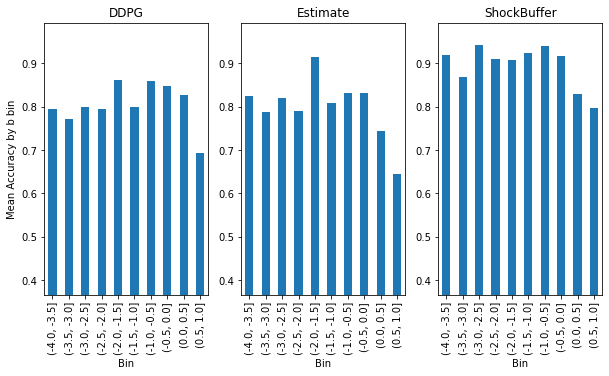
\includegraphics[width=1\textwidth,height=6cm]{figures/Results/bA.png}
  \caption[B Analysis]{Risk aversion analysis } \label{fig:results:bA}
\end{figure}



\section{DDPG Hyper Parameter Analysis}
\subsection{$\tau$ - Target Parameters Learning Rate}
The target network is updated periodically with the parameters from the main network. The rate, $\tau$ at which the target network is updated is controlled by a hyperparameter known as the target network learning rate. A low value for $\tau$ means that the target network parameters are updated slowly, which can help to stabilize the learning process. On the other hand, a high value for $\tau$ means that the target network parameters are updated quickly, which can lead to faster convergence but may also lead to instability in the learning process.  

\subsubsection{Adaptive tau}
 We can set $\tau$ to be high for faster convergence in the beginning of the experiments while reducing it gradually over time to stabilize the process. Sample plots from our experiments showing the representative effect is shown in the 
Figure \ref{fig:tau_analysis}. In the Tau\_Adaptive case, the initial value of $\tau$ is multiplied in  by the factor $(TotalEpisodes-currentEpisode)/TotalEpisodes$ before each update

\begin{figure}[!tbp]
  \centering
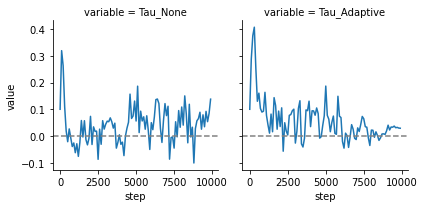
\includegraphics[width=1\textwidth,height=0.2\textheight]{figures/AdaptiveTau.png}
  \caption{$\tau$ analysis for 2 similar experiments}\label{fig:tau_analysis}
\end{figure}
\break
We tried to conduct experiments for studying the effects of adaptive $\tau$ based on the formula we earlier described. We present the configuration of these experiments in Table \ref{table:config_Tau} and the results in Figure \ref{fig:results:tau}
\begin{table}[]
\caption{Configuration - Tau Analysis} \label{table:config_Tau}
\begin{tabular}{||p{3cm}|p{2cm}||p{2cm}|p{2cm}||p{2cm}|p{2cm}||}
\hline
\textbf{Environment Parameter} & \textbf{Sampled values} &\textbf{DDPG}\linebreak \textbf{Parameter}& \textbf{Values} &\textbf{DDPG}\linebreak \textbf{Parameter} & \textbf{Values}\\
\hline

$\mu \in [0,1]$          & [0.07,0.955] & Version & DDPG, Shock Buffer, Estimates & Batch Size          & 1024 \\
\hline
$\sigma \in [0,1]$       & [0.1,1.0] & Grid Points &20 (Estimate)& Batch Size Growth & None \\
\hline
\Delta t          & 0.2 & Shock Buffer Size & 8 (Shock Buffer)& &\\
\hline
$v_0$        & 1 & Noise \linebreak  Decay       & Linear & & \\
\hline
Utility     & power  & Noise \linebreak  Scale       & 1 &&  \\
\hline
$b \in [-10,1) \backslash \{0\}$ & [-10,1) & $\tau$& $5.10^{-4}$ && \\
\hline
            &  & \textbf{Tau Decay}         & \textbf{None and Linear} && \\
\hline
            $r_c$&0  & Buffer Length     & $10^{4}$ && \\
\hline
\end{tabular}
\end{table}


\begin{figure}[!tbp]
     \subfloat[Box plot Analysis Tau ][Box plot analysis - $\tau$ ]{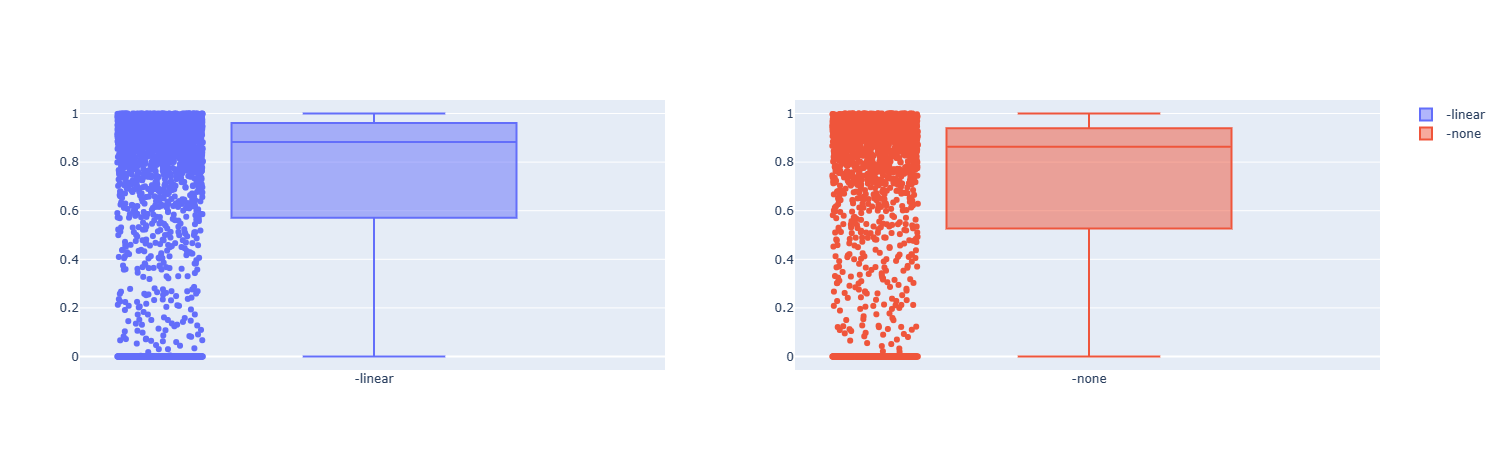
\includegraphics[width=1\textwidth,height=0.22\textheight]{figures/Results/Tau.png}}
  \vfill
  \subfloat[Table analysis Tau ][Table analysis  - $\tau$ ]{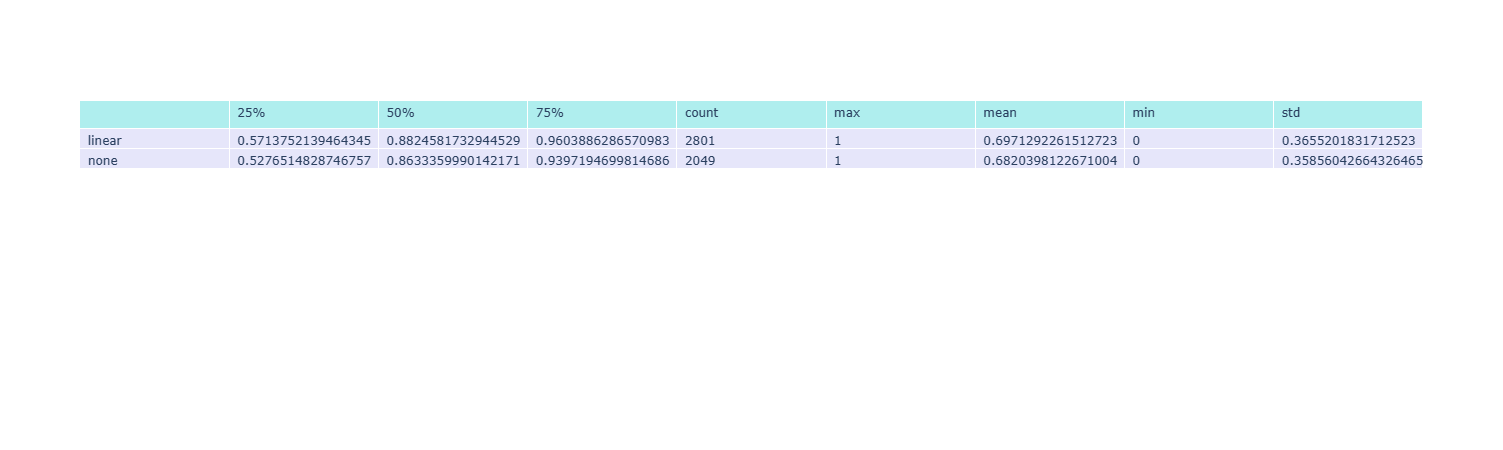
\includegraphics[width=1\textwidth,height=0.22\textheight]{figures/Results/Taudf.png}}
  
  \caption{ $\tau$ analysis}
  \label{fig:results:tau}
\end{figure}
 We noted that having an adaptive policy for tau decay has a positive effect in our experiments.
 \pagebreak
\subsection{Noise Process}

In our experiments, to model the exploration policy while arriving at the optimal action we used the Ornstein Uhlenbeck Process \cite{uhlenbeck1930} as stated in the original paper to generate correlated noise.
In the i-th training step, the noise level $X_i$ is updated recursively through the equation
\begin{equation}\label{equation:ounoise}
    X_i= (1-\kappa\Delta_N) X_{i-1}
    + \sigma_N \sqrt{\Delta_N}\mathcal{N},
\end{equation}

for positive constants $\kappa,\Delta_N,\sigma_N$  and $\mathcal{N} \sim \mathcal{N}(0,1)$.
In our experiments we set $\sigma_N = 0.2$ (volatility of the noise process). $\kappa = 0.15$ (rate at which $X$ reverts to the mean) and $\Delta_N=0.2$

For every call to the noise object specified in Algorithm \ref{alg:eventloop},we update the noise level as per (\ref{equation:ounoise}). Then the noise level is scaled according to an additional hyper parameter. Morever, we have another hyper parameter that decays the whole noise level as we progress on an experiment. Finally we add the resulting noise level to the estimated optimal action, $a^{\phi}$ which we compute at every step. This whole procedure is shown in Algorithm \ref{alg:NoisePolicy}.

\begin{algorithm}
\caption{Noise process - Hyper parameter tuning}
\label{alg:NoisePolicy}
\begin{algorithmic}[1]
\Require
\Statex $currentEpisode,TotalEpisodes$
\Statex $scale,decay$ \Comment{scale is a numeric hyperparameter, decay is a boolean hyperparameter to linearly decay the noise level }
\Statex $noiseLevel,\theta,\mu,\sigma,\Delta t$ \Comment{Parameters of the OU process, $\Delta t$ is the time step}
\Statex $currentEpisode,TotalEpisodes$

\Statex
\State  $noiseLevel \gets \left(
            noiseLevel 
            *(1-\kappa\Delta_N) 
    + \sigma_N \sqrt{\Delta_N}*StandardNormalVariable() 
        \right)$
\State Store $noiseLevel$
\State $decayFactor \gets 1$
\If{$decay = True$}
    \State $decayFactor = (TotalEpisodes-currentEpisode)/TotalEpisodes$
\EndIf
\State \Return {$decayFactor*scale*noiseLevel$}

\end{algorithmic}
\end{algorithm}

By increasing the $scale$  hyper parameter, we can control the exploration part in seeking the optimal action, and by setting $decay$ to True, we can achieve better convergence (while also allowing for high exploration in the beginning of the experiment). These effects are illustrated in Figure \ref{fig:noise_analysis}.

\begin{figure}[H]
  \centering
  \subfloat[Noise low ][Noise factor 0.1]{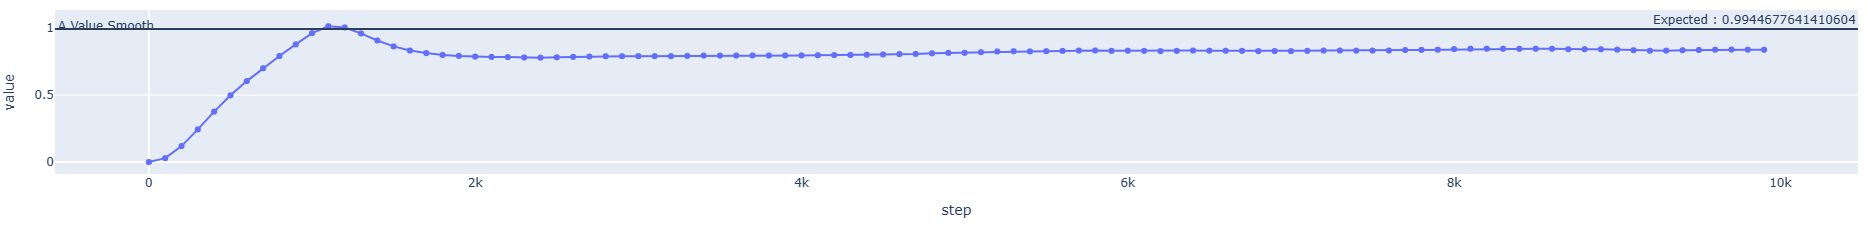
\includegraphics[width=1\textwidth,height=0.2\textheight]{figures/noise_scale_01.png}\label{fig:noise_low}}
  \vfill
  \subfloat[Noise high][Noise factor 5]{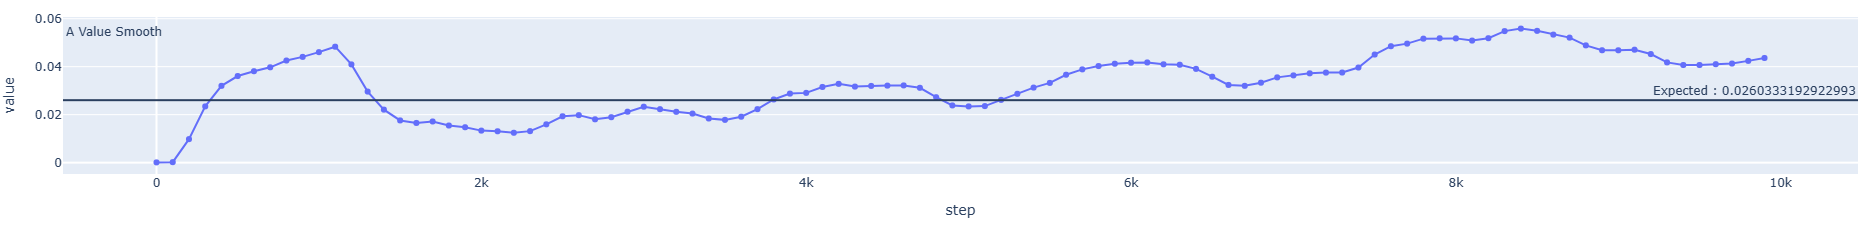
\includegraphics[width=1\textwidth,height=0.2\textheight]{figures/noise_high.png}\label{fig:noise_high}}
  \vfill
    \subfloat[Noise Adaptive][Adaptive noise]{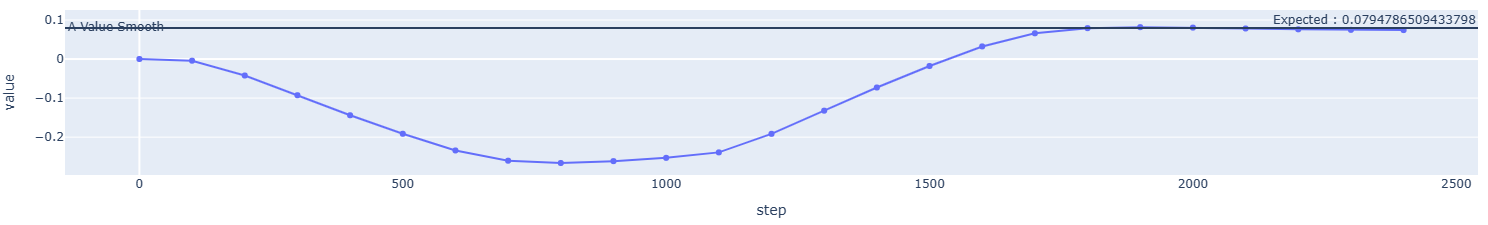
\includegraphics[width=1\textwidth,height=0.2\textheight]{figures/AdativeNoise.png}\label{fig:noise_adaptive}}
  \caption{Noise scale analysis to illustrate effects on convergence and accuracy}
  \label{fig:noise_analysis}
\end{figure}

We conducted a batch of experiments to study the effect of noise scale on the performance, the configuration of the experiments is shown in Table \ref{table:config_noise} and the corresponding results are shown in Figure \ref{fig:results:ns}.

\begin{table}[]
\caption{Configuration - Noise scale Analysis } \label{table:config_noise}
\begin{tabular}{||p{3cm}|p{2cm}||p{2cm}|p{2cm}||p{2cm}|p{2cm}||}
\hline
\textbf{Environment Parameter} & \textbf{Sampled values} &\textbf{DDPG}\linebreak \textbf{Parameter}& \textbf{Values} &\textbf{DDPG}\linebreak \textbf{Parameter} & \textbf{Values}\\
\hline

$\mu \in [0,1]$          & [0.02,0.42] & Version & Shock Buffer& Batch Size          & 1024 \\
\hline
$\sigma \in [0,1]$       & [0.35,0.98] & Grid Points &- & Batch Size Growth & None \\
\hline
\Delta t          & 0.2 & Shock Buffer Size & 8 (Shock Buffer)& &\\
\hline
$v_0$        & 1 & Noise \linebreak  Decay       & Linear & & \\
\hline
Utility     & power, log  & \textbf{Noise scale}       & \textbf{\{0.1,1,2,5\}} &&  \\
\hline
$b \in [-10,1) \backslash \{0\}$ & [-8.1,0.73] & $\tau$& $5.10^{-4}$ && \\
\hline
            T&1  &$\tau$ decay         & Linear && \\
\hline
            $r_c$&0  & Buffer Length     & $10^{4}$ && \\
\hline
\end{tabular}
\end{table}

\begin{figure}[H]
    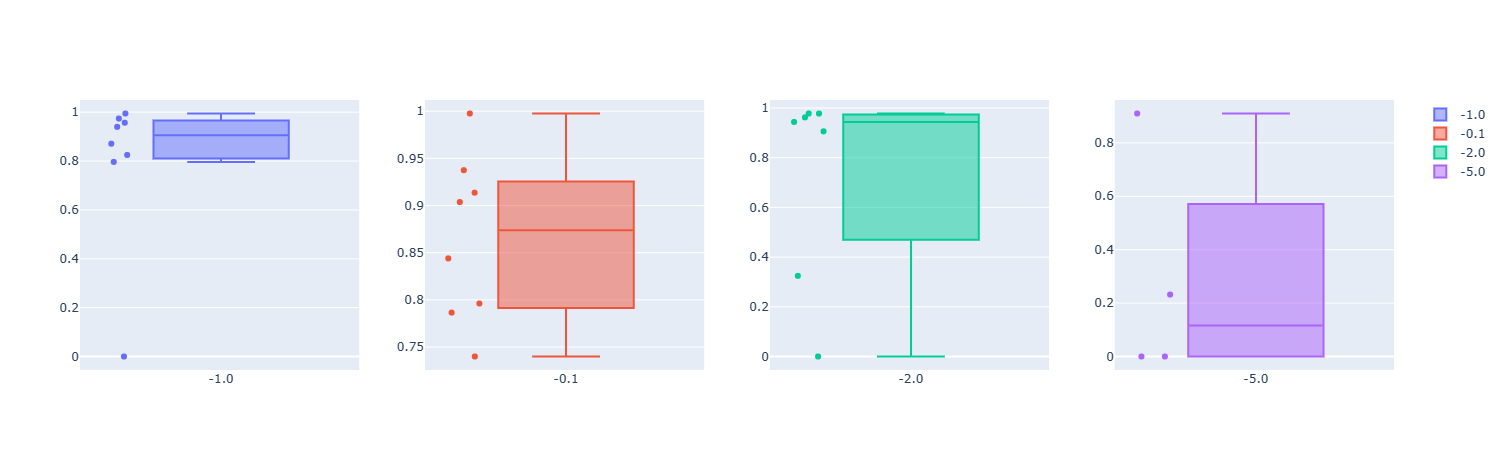
\includegraphics[width=1\textwidth,height=6cm]{figures/Results/NoiseScale.png}
  \caption[Noise scale]{Noise scale Analysis } \label{fig:results:ns}
\end{figure}

We noted that in our experiments having a higher or lower noise scale to increase/decrease our exploration generally did not improve our performance for the configuration we tested.
\pagebreak

\subsection{Episodes}
Typically, we would expect that as we increase the number of episodes, the algorithm should converge. If we observe that the algorithm does not converge it could be mainly because of 2 reasons in our set up (assuming $\tau$ is not decayed).
\begin{itemize}
    \item Approximation for the expectation in the equation (\ref{eq:BMO1}) is too inaccurate (which we discussed in depth in earlier Chapters \ref{chapter:ShockBuffer} and \ref{chapter:Estimates})
    \item The Bellman equation cannot be fitted in a stable manner 
\end{itemize}
\begin{figure}[!tbp]
     \subfloat[Good Covergence ][Good convergence ]{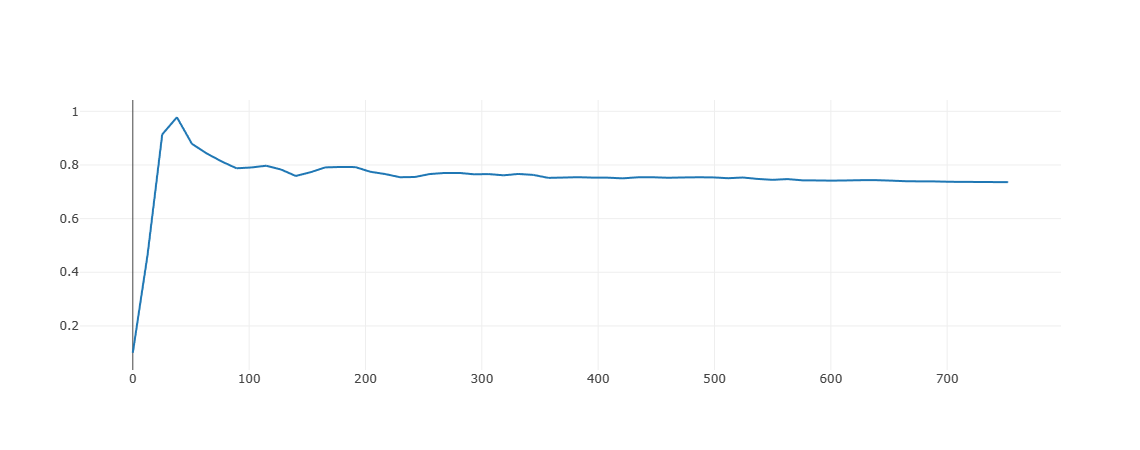
\includegraphics[width=1\textwidth,height=0.22\textheight]{figures/Results/GoodConvergence.png}}
  \vfill
  \subfloat[No convergence ][No Convergence ]{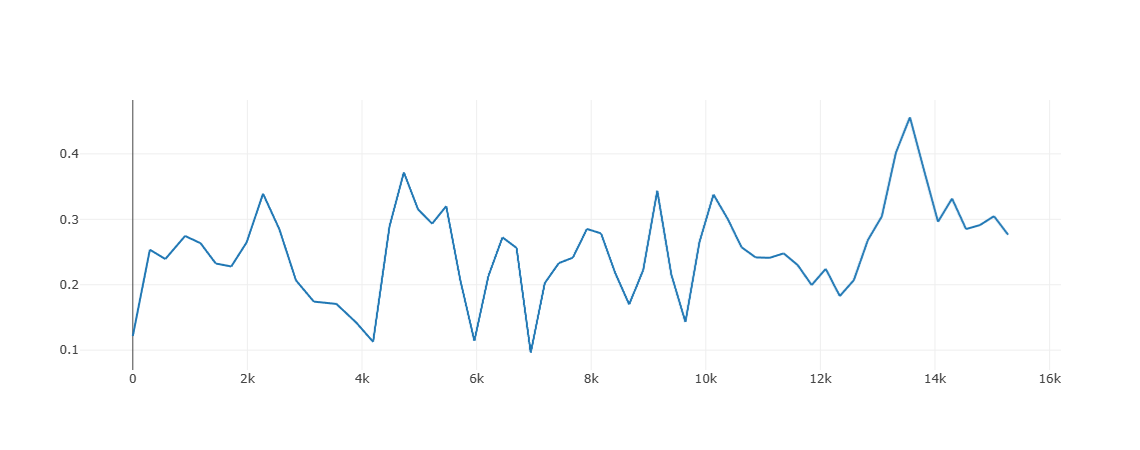
\includegraphics[width=1\textwidth,height=0.22\textheight]{figures/Results/NoConvergence.png}}
  
  \caption{ Episode hyperparamter - to show the solution either converging  or not in our experiments}
  \label{fig:episdode_analysis}
\end{figure}
\pagebreak
When we do not decay $\tau$, or noise over time, we see both good convergence and poor convergence in our experiments. This is shown in Figure \ref{fig:episdode_analysis} - all other parameters of the 2 experiments except $\mu$ and $\sigma$ were identical and yet the convergence was quite different.

We conducted experiments to analyse the effects of the number of episodes. The configuration of these experiments are provided in Table \ref{table:config_episodes} and the results in Figure \ref{fig:results:episodes_analysis_all}.
\begin{table}[]
\caption{Configuration - Number of episodes analysis } \label{table:config_episodes}
\begin{tabular}{||p{3cm}|p{2cm}||p{2cm}|p{2cm}||p{2cm}|p{2cm}||}
\hline
\textbf{Environment Parameter} & \textbf{Sampled values} &\textbf{DDPG}\linebreak \textbf{Parameter}& \textbf{Values} &\textbf{DDPG}\linebreak \textbf{Parameter} & \textbf{Values}\\
\hline

$\mu \in [0,1]$          & [0.016,0.62] & Version & Shock Buffer and Estimates& Batch Size          & 1024 \\
\hline
$\sigma \in [0,1]$       & [0.27,0.98] & Grid Points &20 (Estimates) & Batch Size Growth & None \\
\hline
\Delta t          & 0.2 & Shock Buffer Size & 8 (Shock Buffer)&\textbf{ Episodes} &\textbf{\{}$\mathbf{2.10^4,4.10^4,}$ \lineabreak $ \mathbf{8.10^4}$\textbf{\}}\\
\hline
$v_0$        & 1 & Noise \linebreak  Decay       & Linear & & \\
\hline
Utility     & power, log  & Noise \linebreak  Scale       & 1.0 &&  \\
\hline
$b \in [-10,1) \backslash \{0\}$ & [-7,0.6] & $\tau$& $5.10^{-4}$ && \\
\hline
            T&1  &$\tau$ decay         & Linear && \\
\hline
            $r_c$&0  & Buffer Length     & $10^{4}$ && \\
\hline
\end{tabular}
\end{table}



    \begin{figure}[H]
  \subfloat[Table analysis ][Table analysis - number of episodes ]{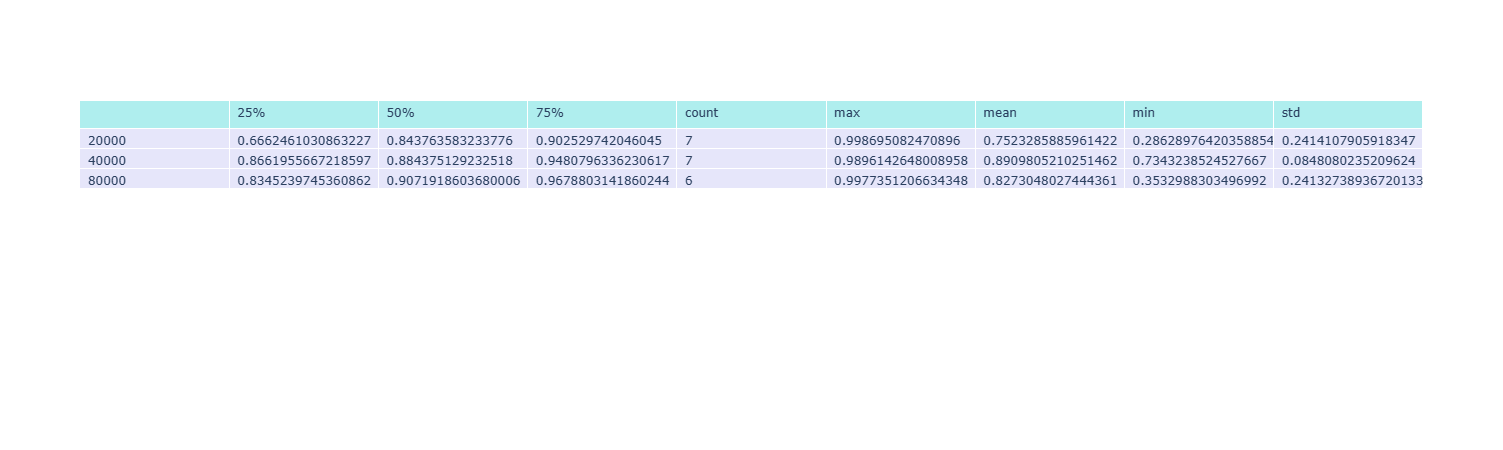
\includegraphics[width=1\textwidth,height=0.22\textheight]{figures/Results/episodes_analysis.png}}
  
  \caption{ Episodes analysis}
  \label{fig:results:episodes_analysis_all}
\end{figure}

We see that when we increase the number of episodes, accuracy does increase (albeit only marginally). For Estimates we did not see any improvement as we increase the number of episodes. When we inspected individual plots, we find out that convergence (even if not to the optimal action) happens fairly early during training. 


\section{Robust Simulations} \label{section:rs}



After our initial experiments, we observed 2 key points.
\begin{itemize}
    \item Increasing the number of episodes only marginally increases the accuracy. We observed the Q loss decreased with episodes but the optimal action was not necessarily maximized.
    \item Shock Buffer and Estimates  performed better in almost all aspects compared to DDPG.
\end{itemize}
So coming up with more accurate expectations in Equation (\ref{eq:BMO1}) helped a long way for having robust simulations. We used this idea and tried to build better estimates by the following methods.

\subsection{Estimates}
We conducted 2 kinds of experiments. 
\begin{itemize}
\item
We created 2 sets of partitions -  coarse and fine over $-\inf,\inf$. We used the fine ones from -0.5 to 0.5 roughly and coarse ones outside of that interval. The reason behind this idea was to build different (and better) partition sets for estimates that would better converge to the expected value. 
\item
\textit{Adaptive partition strategy}: We started  off with very fine partitions (around 200) to begin with and then increased over time.
\end{itemize}
However we noted that both these experiments did not improve the accuracy by much. Then we decided on a brute force solution and merely increased the number of grid points, i.e "m", to a very high number - increased from 20 to 1000. We kept the number of episodes to 2500 as we observed that convergence happens rapidly in Estimates. We also built our solution on GPUs to help us cope with the memory constraints such a configuration would entail.

\subsection{Shock Buffer}

We followed a very similar strategy for Shock Buffer. However, as we observed that Shock Buffer took longer to converge, we increased the number of episodes to 6000, while increasing the mini batch size $m=B_p$ for log returns from 20 to 1000.
\pagebreak
\subsection{Results}
We then ran these configurations on both power and log utility functions and repeated the experiment under different market parameters. We display the configuration of these experiments in Table \ref{table:config_env} and the results in Figure \ref{fig:results:M}.

\begin{table}[]
\caption{Configuration - M Analysis} \label{table:config_env}
\begin{tabular}{||p{3cm}|p{2cm}||p{2cm}|p{2cm}||p{2cm}|p{2cm}||}
\hline
\textbf{Environment Parameter} & \textbf{Sampled values} &\textbf{DDPG}\linebreak \textbf{Parameter}& \textbf{Values} &\textbf{DDPG}\linebreak \textbf{Parameter} & \textbf{Values}\\
\hline

$\mu \in [0,1]$          & [0.07,0.955] & Version & DDPG, Shock Buffer, Estimates & Batch Size          & 1024 \\
\hline
$\sigma \in [0,1]$       & [0.1,1.0] & Grid Points &\textbf{1000} (Estimates)& Batch Size Growth & None \\
\hline
\Delta t          & 0.2 & Shock Buffer Size & \textbf{1000} (Shock Buffer)& Episodes& \textbf{Estimates: 2500   \lineabreak Shock Buffer: 6000 }\\
\hline
$v_0$        & 1 & Noise \linebreak  Decay       & Linear & & \\
\hline
Utility     & power and log & Noise \linebreak  Scale       & 1 &&  \\
\hline
$b \in [-10,1) \backslash \{0\}$ & [-9.0,0.95] & $\tau$& $5.10^{-4}$ && \\
\hline
            T&1  &$\tau$ decay         & Linear && \\
\hline
            $r_c$&0  & Buffer Length     & $10^{4}$ && \\
\hline
\end{tabular}
\end{table}
\begin{figure}[!tbp]
     \subfloat[Box plot Analysis M ][Box plot analysis - m ]{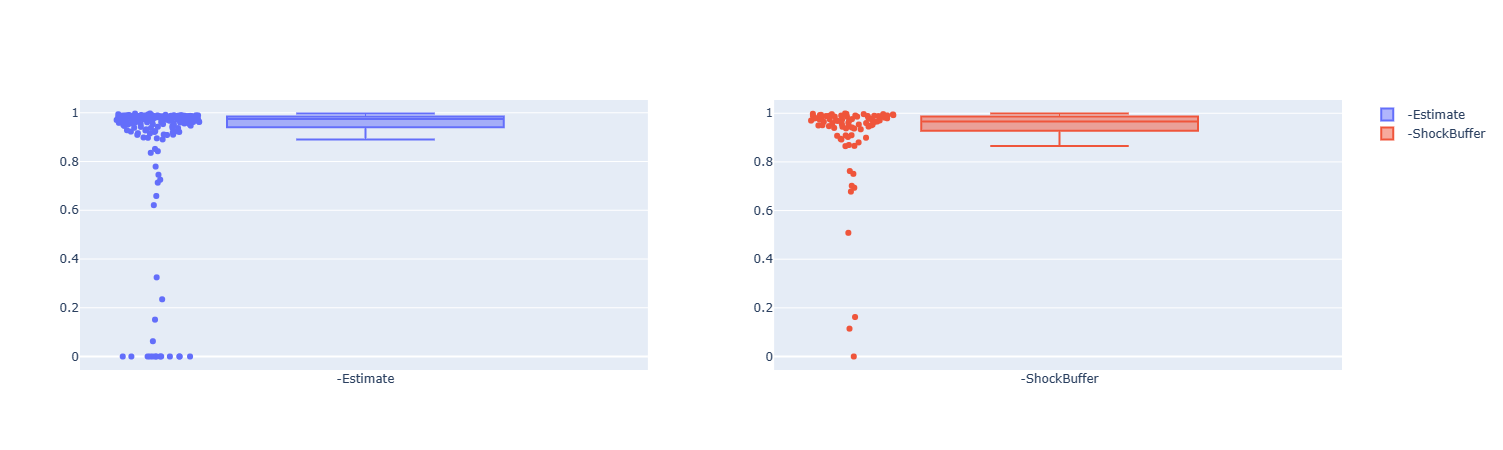
\includegraphics[width=1\textwidth,height=0.22\textheight]{figures/Results/Accuracy_M.png}}
  \vfill
  \subfloat[Table analysis M ][Table analysis estimates - m]{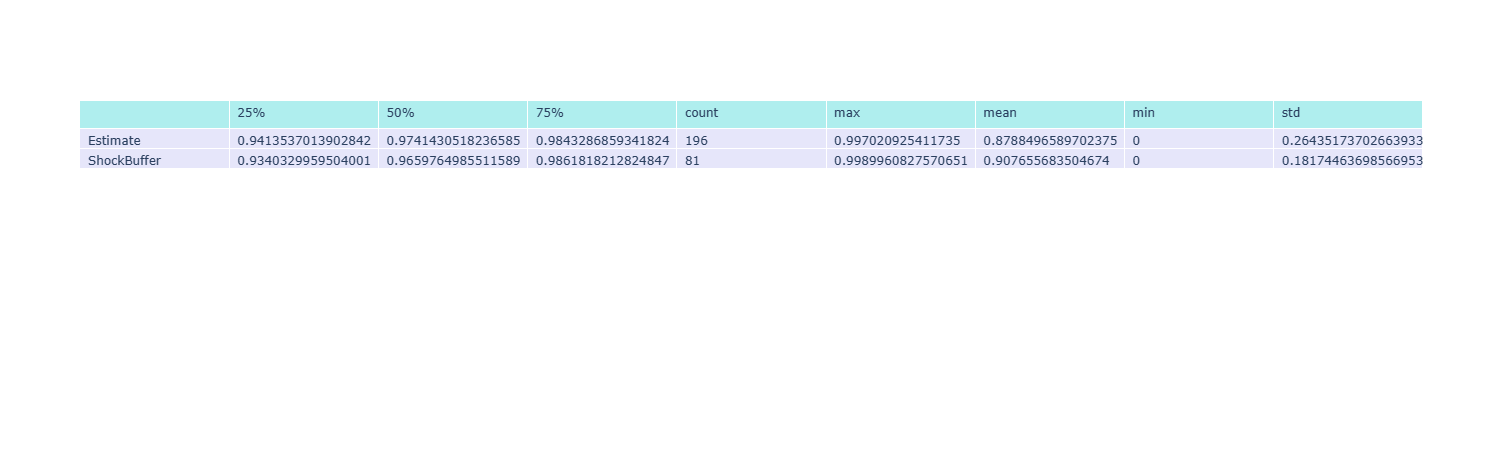
\includegraphics[width=1\textwidth,height=0.22\textheight]{figures/Results/Accuracy_M_df.png}}
  
  \caption{ $m$ analysis}
  \label{fig:results:M}
\end{figure}


We observed that this version of both these algorithm performed comparatively better, even we decreased $\Delta t$ from 0.2 to 0.01. The results for $\Delta t = 0.01$ (other configuration parameters are the same) are shown in Figure \ref{fig:results:ML}


\begin{figure}[!tbp]
     \subfloat[Box plot Analysis M (large timesteps) ][Box plot analysis m ]{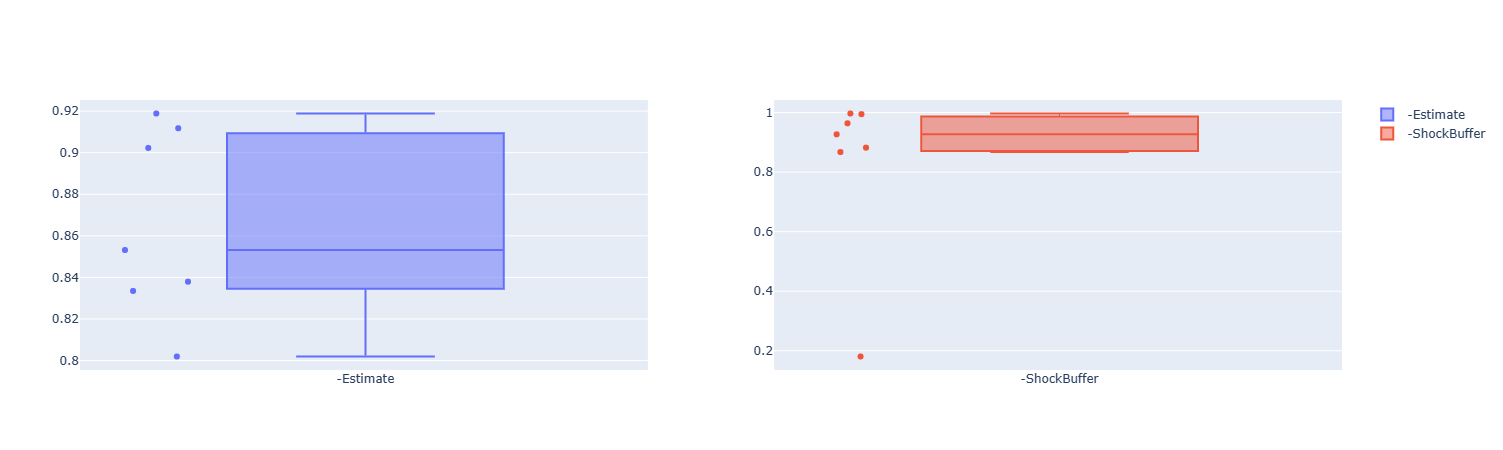
\includegraphics[width=1\textwidth,height=0.22\textheight]{figures/Results/Accuracy_M_long.png}}
  \vfill
  \subfloat[Table analysis M (large timesteps)][Table analysis estimates - m ]{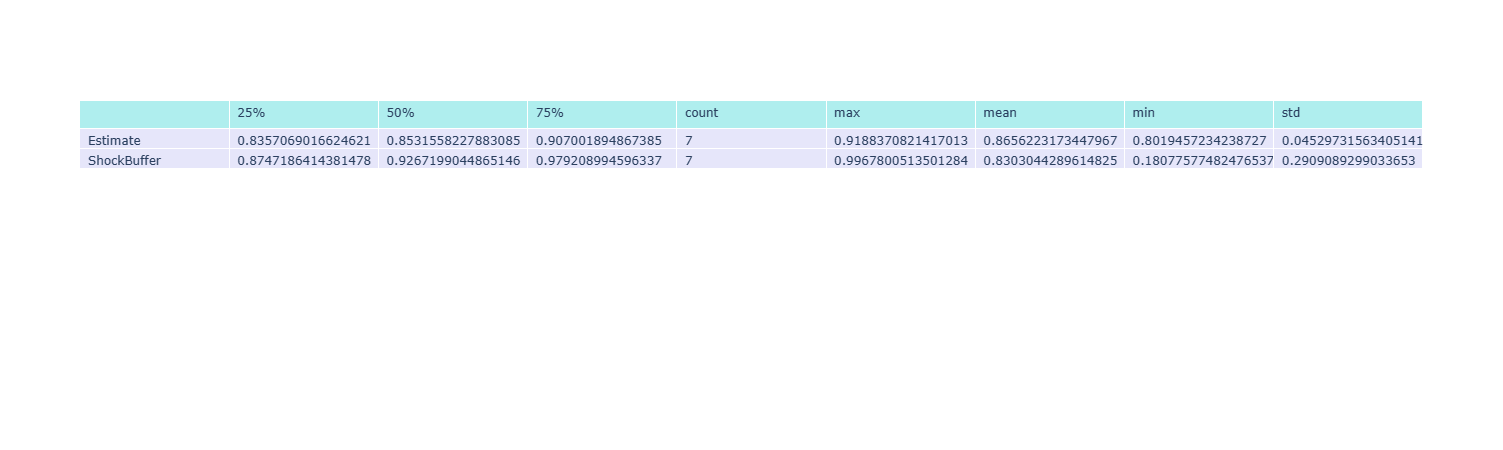
\includegraphics[width=1\textwidth,height=0.22\textheight]{figures/Results/Accuracy_M_df_long.png}}
  
  \caption{ $m$ analysis - $\Delta t$ - 0.01}
  \label{fig:results:ML}
\end{figure}

These results are much better than our initial analysis. It does appear that Shock Buffer is better compared to the Estimates. However, we also note that Estimates is much faster (around 3 times faster) than Shock Buffer in the above set up.  Further, we notice that as we keep increasing the number of grid points, the accuracy of Estimates also increases. Hence, Estimates, in a sense, can be regarded as equivalent to the Shock Buffer. 

Another interesting pattern we found was that Estimates performed much better for log utility functions than for power utility functions. However, we could not find such a pattern for  Shock Buffer. This pattern is captured in Figure \ref{fig:results:EstimatesU2} and \ref{fig:results:SBU2}

\begin{figure}[!tbp]
     \subfloat[Box plot Analysis - Estimates for Utility functions  ][Box plot Analysis - Estimates for log and power utility functions ]{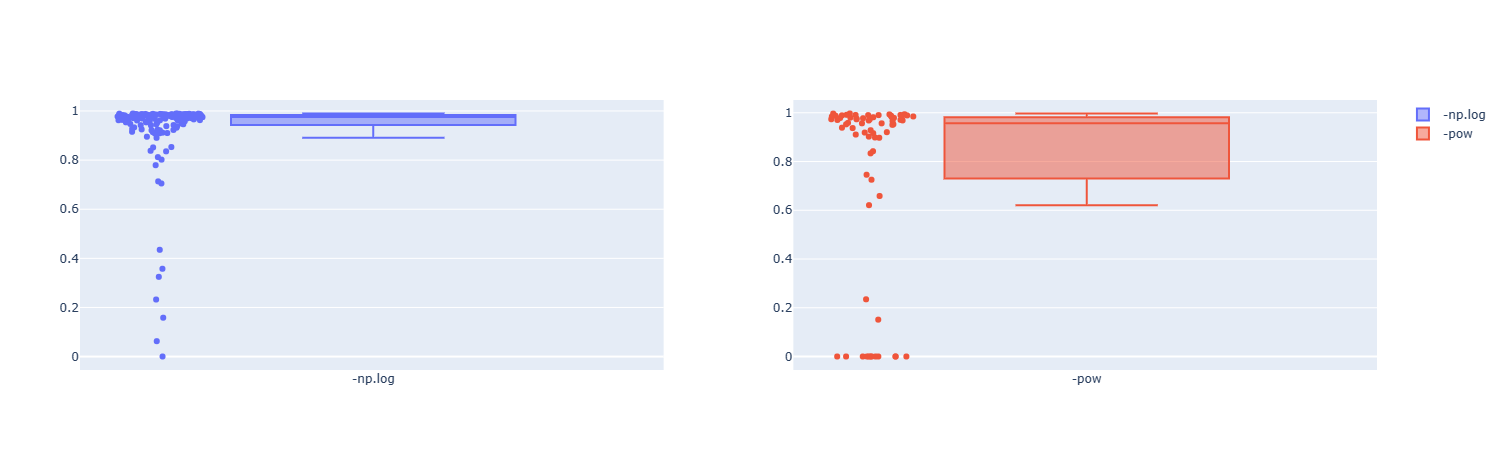
\includegraphics[width=1\textwidth,height=0.22\textheight]{figures/Results/Accuracy_MEU2.png}}
  \vfill
  \subfloat[Table analysis - Estimates for Utility functions ][Table analysis Estimates for log and power utility functions ]{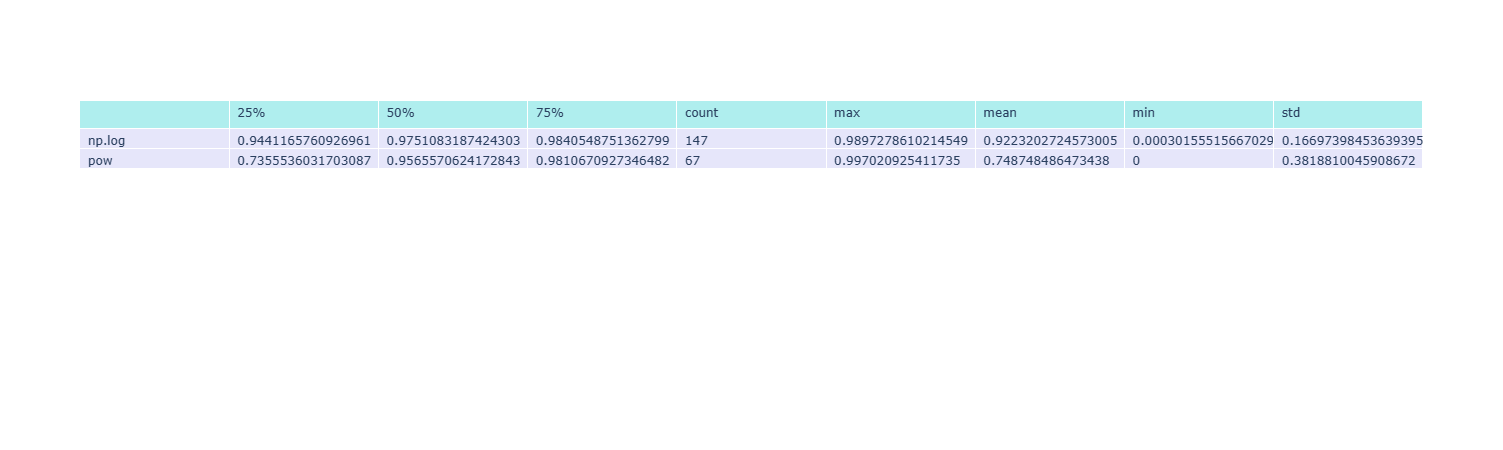
\includegraphics[width=1\textwidth,height=0.22\textheight]{figures/Results/Accuracy_MEU2_df.png}}
  
  \caption{ Utility functions analysis - Estimates}
  \label{fig:results:EstimatesU2}
\end{figure}


\begin{figure}[!tbp]
     \subfloat[Box plot Analysis - Shock Buffer for Utility functions  ][Box plot Analysis - Shock Buffer for log and power utility functions ]{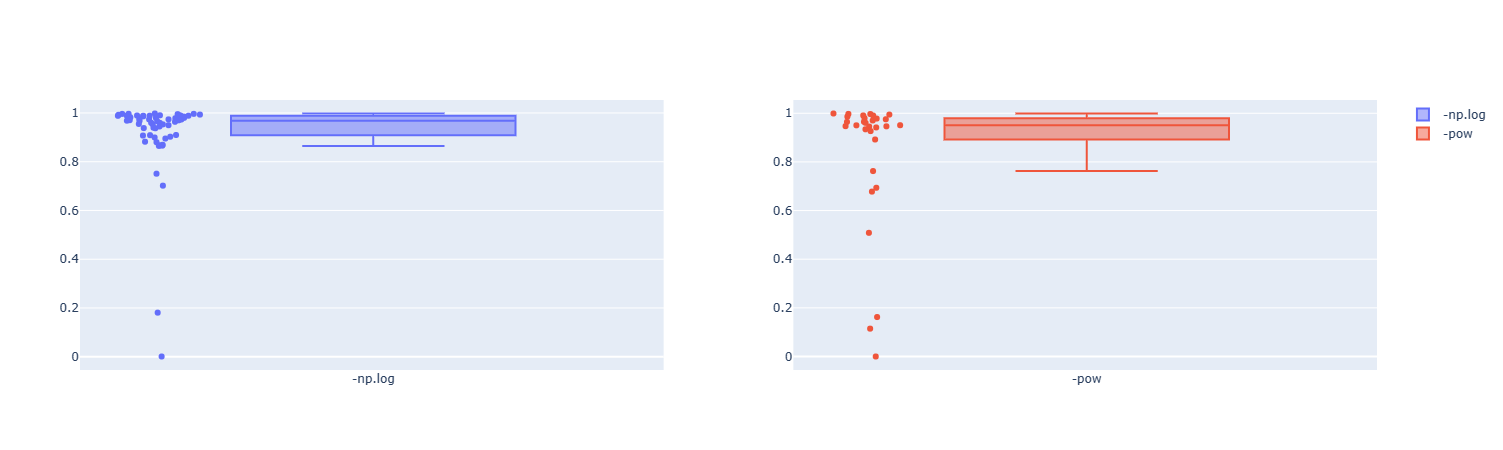
\includegraphics[width=1\textwidth,height=0.22\textheight]{figures/Results/Accuracy_MEU2SB.png}}
  \vfill
  \subfloat[Table analysis - Shock Buffer for log and power utility functions ][Table analysis Shock Buffer for log and power utility functions ]{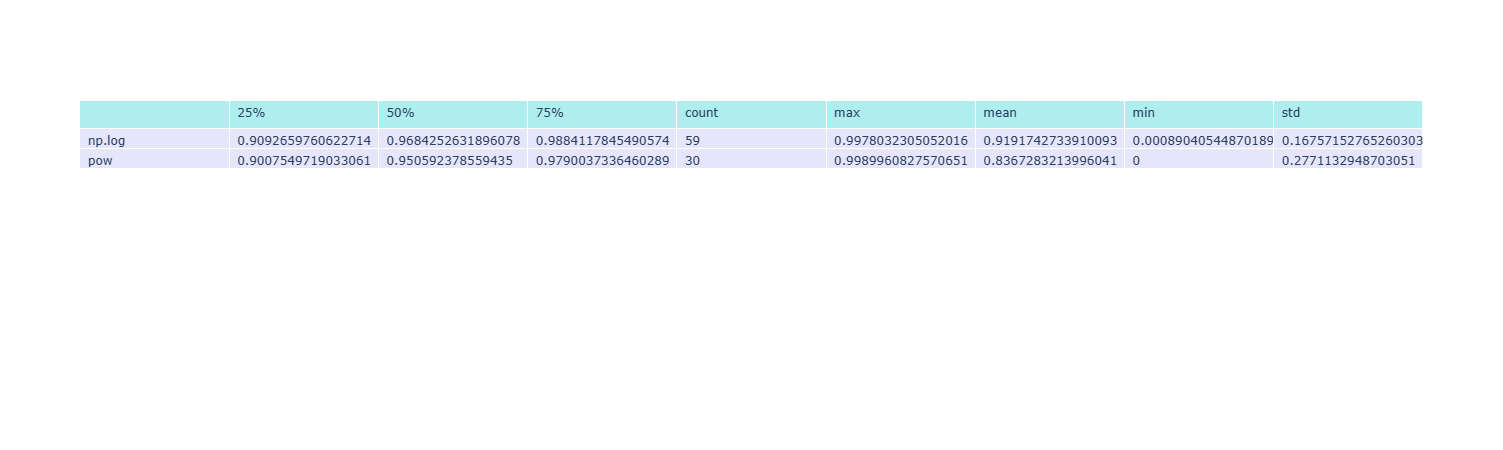
\includegraphics[width=1\textwidth,height=0.22\textheight]{figures/Results/Accuracy_MEU2_dfSB.png}}
  
  \caption{ Utility functions analysis - Shock Buffer}
  \label{fig:results:SBU2}
\end{figure}







